\uuid{nxy8}
\exo7id{5472}
\auteur{rouget}
\organisation{exo7}
\datecreate{2010-07-10}
\isIndication{false}
\isCorrection{true}
\chapitre{Intégration}
\sousChapitre{Intégrale de Riemann dépendant d'un paramètre}

\contenu{
\texte{
Etude de $f(x)=\int_{-1}^{1}\frac{\sin x}{1-2t\cos x+t^2}\;dt$.
}
\reponse{
Notons $D$ le domaine de définition de $f$.

Si $x\in D$, $-x\in D$ et $f(-x)=-f(x)$. $f$ est donc impaire.

Si $x\in D$, $x+2\pi\in D$ et $f(x+2\pi)=f(x)$. $f$ est donc $2\pi$-périodique.

On étudiera donc $f$ sur $[0,\pi]$.

Soient $x\in[0,\pi]$ et $t\in[-1,1]$. $t^2-2t\cos x+1=(t-\cos x)^2+\sin^x\geq0$ avec égalité si et seulement si $\sin x=0$ et $t-\cos x=0$.

Ainsi, si $x\in]0,\pi[$, $\forall t\in]-1,1[,\;t^2-2t\cos x+1\neq0$. On en déduit que la fraction rationnelle $t\mapsto
\frac{\sin t}{1-2t\cos x+t^2}$ est continue sur $[-1,1]$, et donc que $f(x)$ existe.

Si $x=0$, $\forall t\in[-1,1[$, $\frac{\sin x}{t^2-2t\cos x+1}=\frac{0}{(t-1)^2}=0$. On prut prolonger cette fonction par continuité en $1$ et consisérer que $f(0)=\int_{-1}^{1}0\;dt=0$. De même, on peut considérer que $f(\pi)=0$.

Ainsi, $f$ est définie sur $[0,\pi]$ et donc, par parité et $2\pi$-périodicité, sur $\Rr$.

Soit $x\in]0,\pi[$.Calculons $f(x)$.

\begin{align*}\ensuremath
f(x)&=\int_{-1}^{1}\frac{\sin x}{(t-\cos x)^2+\sin^2x}\;dt=\left[\Arctan\frac{t-\cos x}{\sin x}\right]_{-1}^{1}
=\Arctan\frac{1-\cos x}{\sin x}+\Arctan\frac{1+\cos x}{\sin x}\\
 &=\Arctan\frac{2\sin^2(x/2)}{2\sin(x/2)\cos(x/2)}+\Arctan\frac{2\cos^2(x/2)}{2\sin(x/2)\cos(x/2)}
=\Arctan(\tan(x/2))+\Arctan(\frac{1}{\tan(x/2)})\\
 &=\frac{\pi}{2}\;(\mbox{car}\;\tan(x/2)>0\;\mbox{pour}\;x\in]0,\pi[).
\end{align*}

Ce calcul achève l'étude de $f$. En voici le graphe~:

$$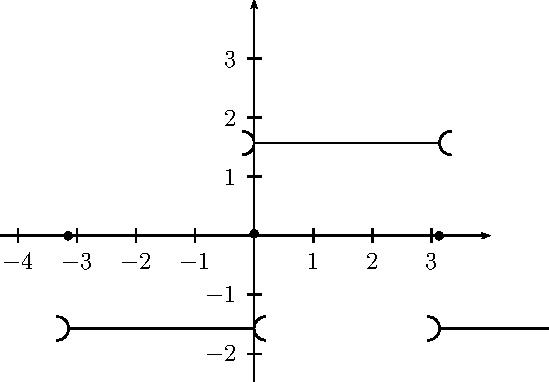
\includegraphics{../images/img005472-1}$$
}
}
